\documentclass[12pt]{ctexart}
\usepackage{amsmath,graphicx,textcomp,subfigure,indentfirst,ctex,color,float}
\usepackage{bm, mhchem}
\title{Lecture 13}
\author{授课、校对:茅奕  \\ 记录:赵思逸}

\date{2022年5月31日}

\newcommand{\refeq}[1]{式~(\ref{#1})}
\newcommand{\refeqs}[2]{式~(\ref{#1}) - (\ref{#2})}
\newcommand{\reffig}[1]{图~\ref{#1}}
\begin{document}

\maketitle

\section{暗物质晕的结构}

暗物质晕内部的密度并不是均匀的。我们可以用一些解析的模型来描述。

\subsection{power-law density profile}

最简单的是 幂律谱模型 (power-law density profile)

\begin{equation}
    \rho(r)=\rho_{0}\left(\frac{r}{r_{0}}\right)^{-\gamma}
\end{equation}
% $$
% \rho(r)=\rho_{0}\left(\frac{r}{r_{0}}\right)^{-\gamma}, \text { with } \gamma=\frac{9 \epsilon}{1+3 \epsilon}
% $$
在半径$r$内的质量
\begin{equation}
    M(<r)=4 \pi \int_{0}^{r} \rho\left(r^{\prime}\right){r^{\prime}}^{2} d r^{\prime}=\frac{4 \pi \rho_{0} r_{0}^{\gamma}}{3-\gamma} r^{3-\gamma}
\end{equation}

当 $\gamma \leq 3$ 时, $\lim _{r \rightarrow \infty} M(<r)=\infty$ ,总质量发散。

当 $\gamma \geq 3$ 时, $\lim_{r \rightarrow 0} M(>r)=\infty$ ,质量在暗物质晕中心发散。 

可见一个幂律谱无法描述暗物质晕的结构,需要 两个幂律谱拼起来,即 double power-law profile.

\subsection{double power-law profile}
我们希望
\begin{equation}
    \begin{cases}\rho \propto r^{-\gamma} & r \ll r_{0} \\ \rho \propto r^{-\beta} & r \gg r_{0}\end{cases}
\end{equation}
数学上给出下式满足条件
\begin{equation} \label{eq:double-pl}
    \rho(r)=\frac{\rho_{0}}{\left(r / r_{0}\right)^{\gamma}\left[1+\left(r / r_{0}\right)^{\alpha}\right]^{(\beta-\gamma) / \alpha}}
\end{equation}
% $\rho(r)=\frac{\rho_{0}}{\left(r / r_{0}\right)^{\gamma}\left[1+\left(r / r_{0}\right)^{\alpha}\right]^{(\beta-\gamma) / \alpha}} \Rightarrow \begin{cases}\rho \propto r^{-\gamma} & r \ll r_{0} \\ \rho \propto r^{-\beta} & r \gg r_{0}\end{cases}$
可以验证
当 $r \ll r_0$ 时,$1+(r/r_0)^\alpha \simeq 1$, \refeq{eq:double-pl} 近似为 $\rho = \rho_0 \left(\frac{r}{r_0}\right) ^{-\gamma}$. 
当 $r \gg r_0$ 时,$1+(r/r_0)^\alpha \simeq (r/r_0)^\alpha$, \refeq{eq:double-pl} 近似为 $\rho = \rho_0 \left(\frac{r}{r_0}\right) ^{-\beta}$.
为了避免 总质量发散或者中心质量发散,
要求
$\gamma < 3$, $\beta > 3$.

\subsection{NFW profile}

我们有了 double power-law profile ,但还不知道 $\alpha, \beta, \gamma$ 三个参数的取值。

N体模拟给出的 NFW profile (由 Navarro, Frenk \& White 发现) 是目前比较常用的一个好的近似模型。
% 它是一个 double power-law 模型, 
NFW profile 取 $\alpha =1$, $\beta=3$, $\gamma =1$,  其表达式为
\begin{equation} \label{eq:NFW}
    \rho(r)=\rho_{\text {crit }} \frac{\delta_{\text {char }}}{\left(r / r_{s}\right)\left(1+r / r_{s}\right)^{2}}
\end{equation}

如 \reffig{fig:NFW}  所示。
\begin{figure}[!hbtp]
	\centering 
	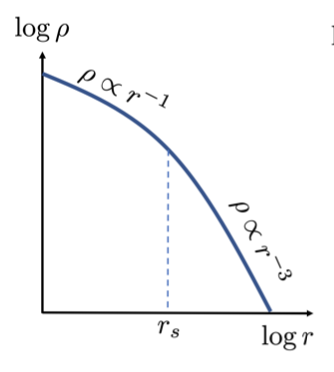
\includegraphics[width=1.0\linewidth]{NFW.png}
	\caption{NFW profile 示意图}
    \label{fig:NFW}
\end{figure}

NFW profile 存在一个问题 : Cusp-Core controversy. 
NFW profile 给出在靠近暗物质晕中心的区域, $\rho \propto r^{-1}$, 有一个高密度的“尖”,即 cusp.
但观测更倾向于 暗物质晕在中心区域密度不变, 即 “核”的结构 (core), $\rho \propto r^0$.
这对 冷暗物质理论提出了挑战。有人认为这说明 冷暗物质模型不对,他们提出了一些候选理论,比如温暗物质(warm dark matter),温暗物质是运动速度比冷暗物质快的一类粒子,这样它就会在暗物质晕形成时将中心密度较大区域的密度差异抹平。另一些人认为观测的是重子物质的分布,有可能重子物质分布和暗物质分布并不相同,重子物质在中心的分布是Core,而暗物质的分布是Cusp.
% ,用来推断

\section{暗物质晕的形成}

暗物质晕的形成也是 bottom-up scenario.
暗物质晕由小质量的晕通过并合逐渐增大的过程叫做 
Merger Tree. 如 \reffig{fig:MegerTree} 所示。

\begin{figure}[!hbtp]
	\centering 
	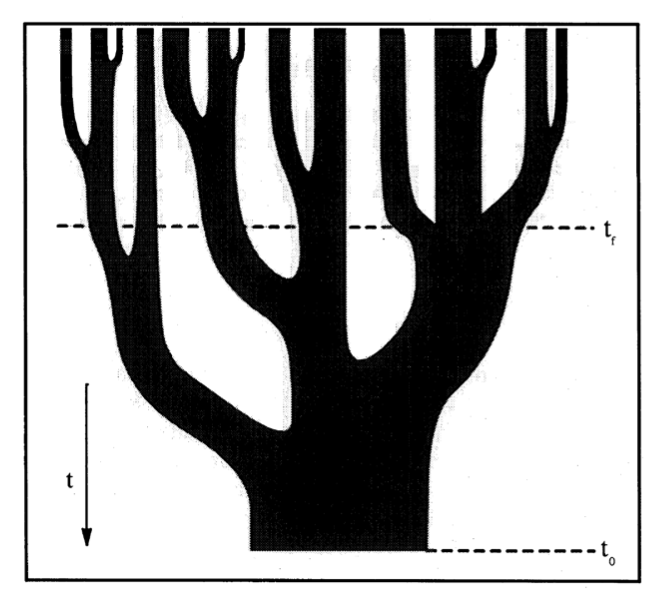
\includegraphics[width=1.0\linewidth]{MegerTree.png}
	\caption{Meger Tree 示意图}
    \label{fig:MegerTree}
\end{figure}

并合的过程也叫做 assembly history ,
assembly history 会影响 暗物质晕的性质,因此是目前重要的研究方向之一。

在暗物质晕的形成中,我们关心不同质量的暗物质晕分别会形成多少。
一个近似的方法是
随机行走 (Random Walk) of dark matter halo statistics.
物质密度的空间分布是随机的,当局部密度大于 临界密度 $\delta_\text{crit}$ 时,我们认为这里形成一个 暗物质晕。 如 \reffig{fig:RandomWalk} 所示,红色标出的区域是大小不同的暗物质晕。

\begin{figure}[!hbtp]
	\centering 
	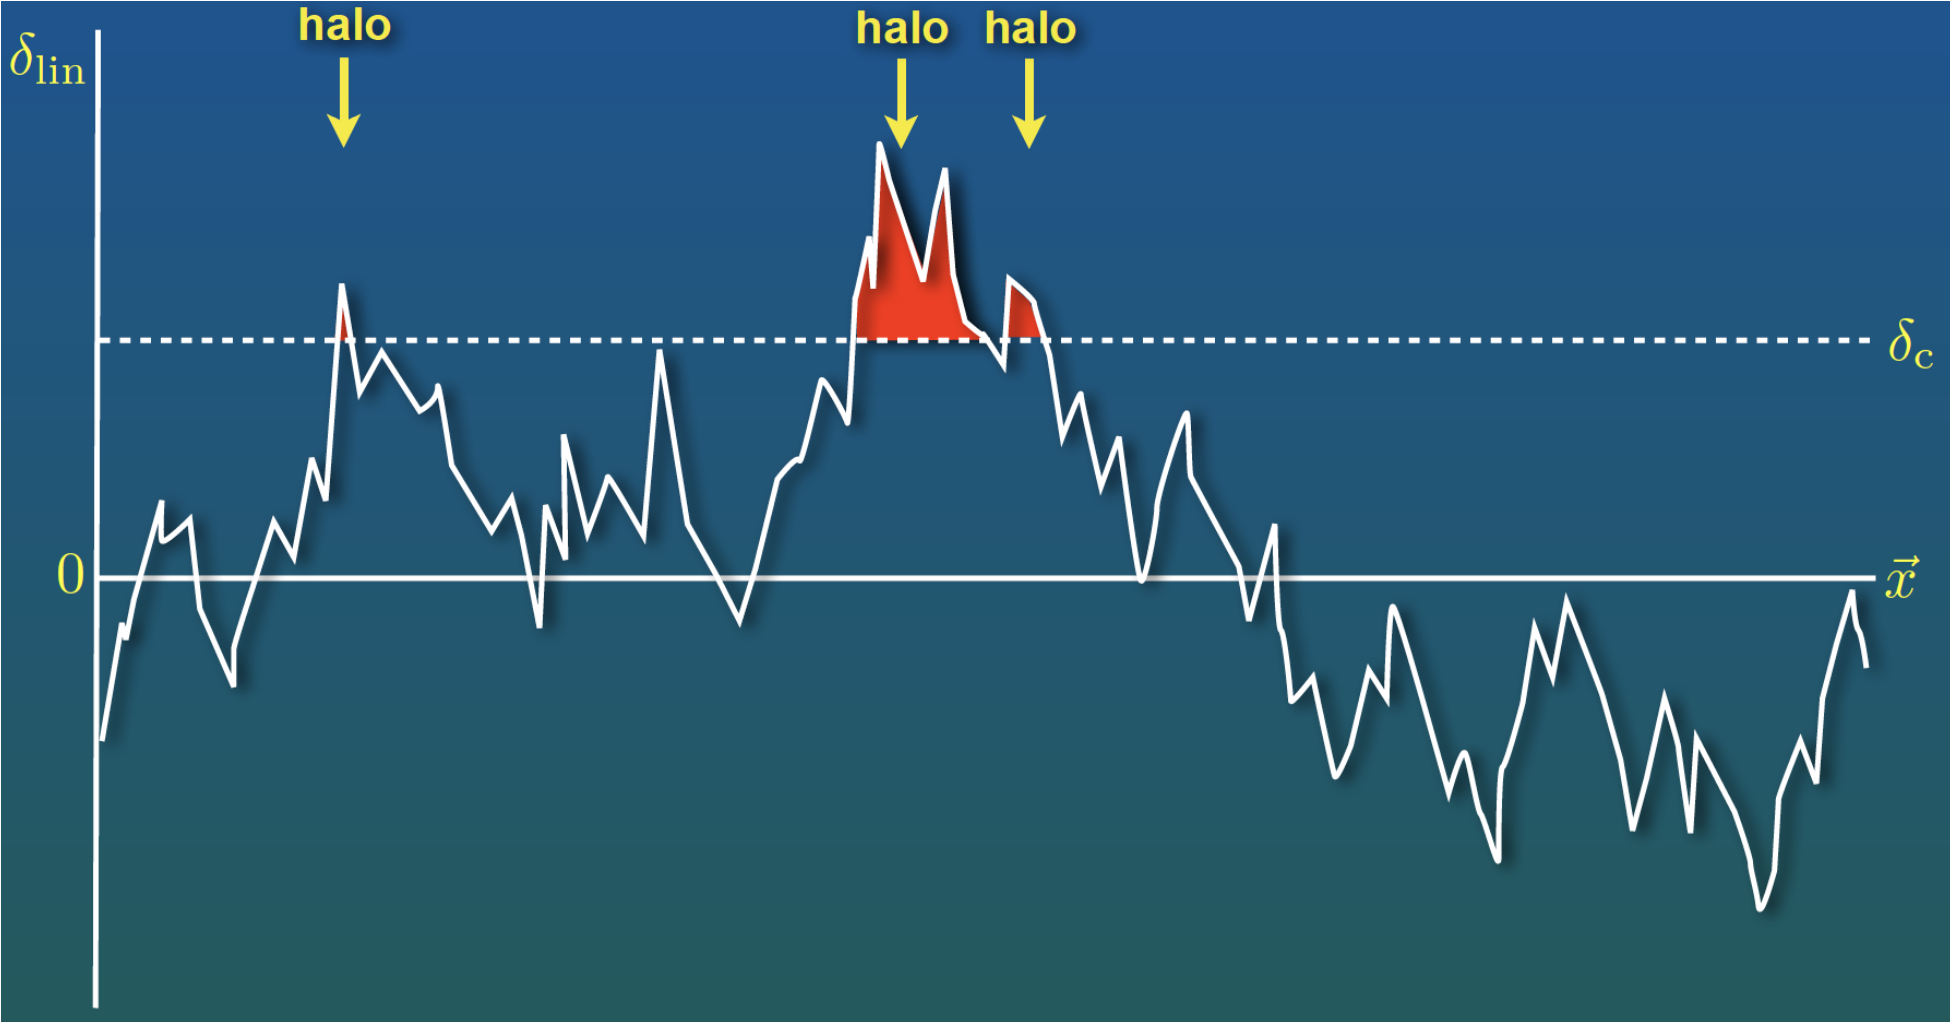
\includegraphics[width=1.0\linewidth]{Peaks_halo.png}
	\caption{Random Walk 示意图}
    \label{fig:RandomWalk}
\end{figure}

在 半径 $R$ 的范围内 对密度涨落做平滑: 
$\delta_M = \delta\left(\vec{x},R\right) $. 
这个平滑尺度对应 质量 $M=\bar{\rho} \times \frac{4}{3} \pi R^3$.

我们想计算 的 halo mass function 是 在一定质量范围内(大于$M$) halo 的数密度,
它 等于
在平滑尺度为 $M$ 时的  峰的 数密度
$n\left(>M\right) = n _{\rm{pk}} \left(\delta_M\right)$ .

Press-Schechter 模型
假设密度场是高斯分布
\begin{eqnarray}
    \mathcal{P}\left(\delta_{M}>\delta_{c}(t)\right) &=& F(>M, t) \\ 
    &=& \frac{1}{\sqrt{2 \pi} \sigma_{M}} \int_{\delta_{c}}^{\infty} \exp \left[-\frac{\delta_{M}^{2}}{2 \sigma_{M}^{2}}\right] d \delta_{M}=\frac{1}{2} \operatorname{erfc}\left[\frac{\delta_{c}}{2 \sigma_{M}}\right]
\end{eqnarray}
其中 $\operatorname{erfc}(x)=1-\operatorname{erf}(x)$, $\operatorname{erf}(x)=\frac{2}{\sqrt{\pi}} \int_{0}^{x} e^{-t^{2}} d t$ 是  error function.

\section{盘星系的形成}

盘星系 (Disk Galaxy) 有盘结构,有些有旋臂,有些有棒状结构。
它的主要亮度集中在盘面上,但一般盘面两侧也有恒星和气体,
单纯只有盘的星系非常少。

\begin{figure}[!hbtp]
	\centering 
	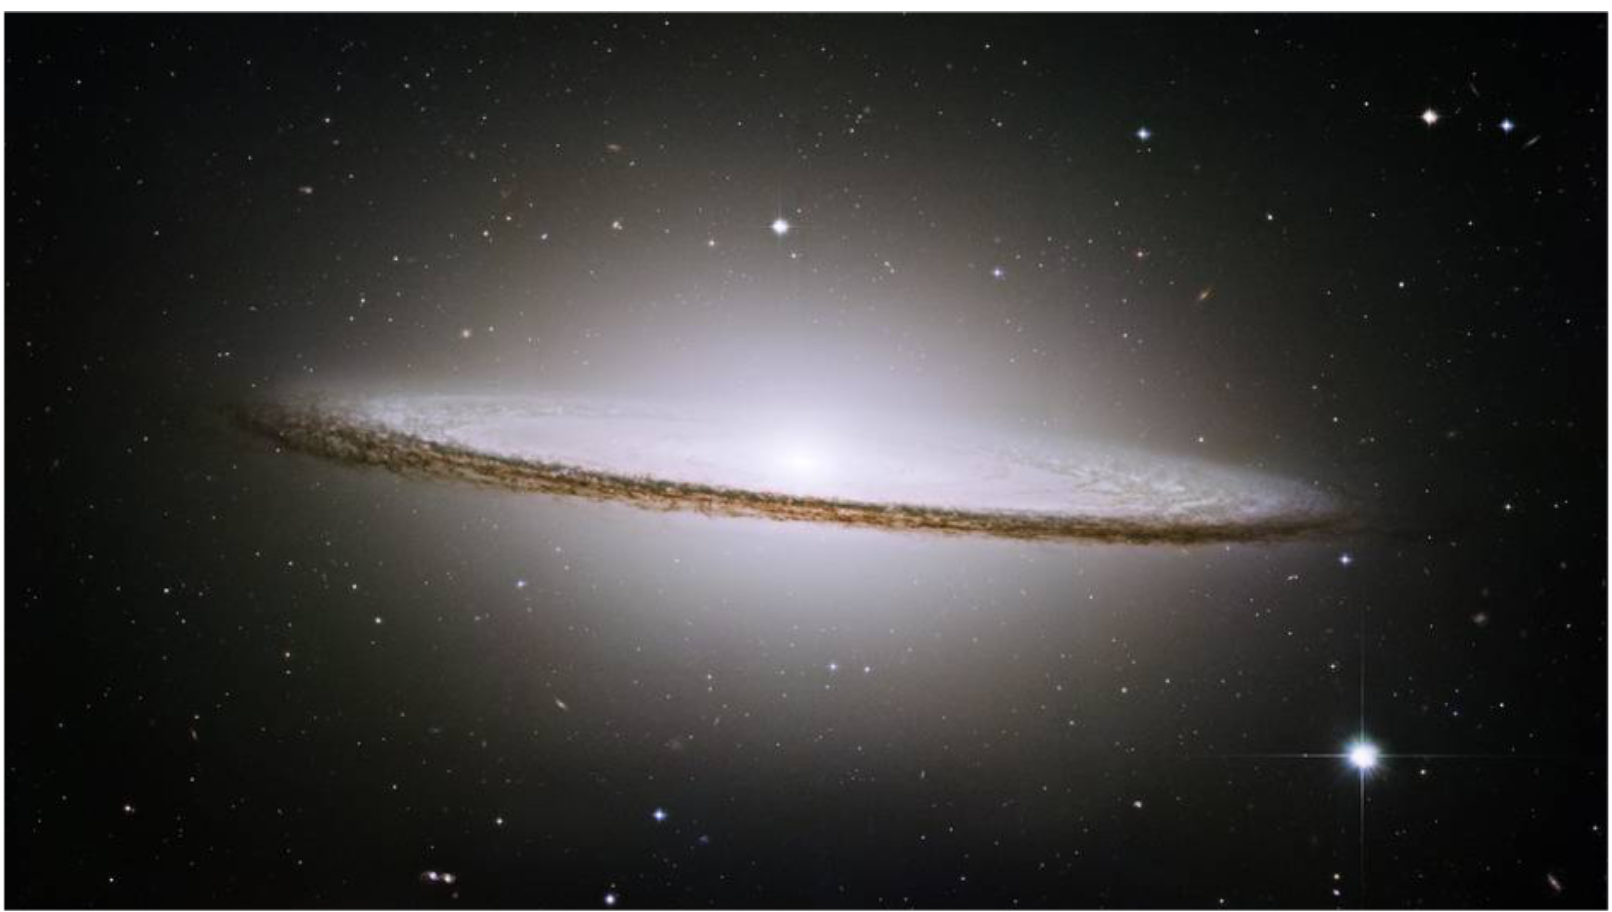
\includegraphics[width=1.0\linewidth]{disk_galaxy.png}
	\caption{典型的盘星系,盘面两侧亦有分布}
    \label{fig:disk}
\end{figure}

\begin{figure}[!hbtp]
	\centering 
	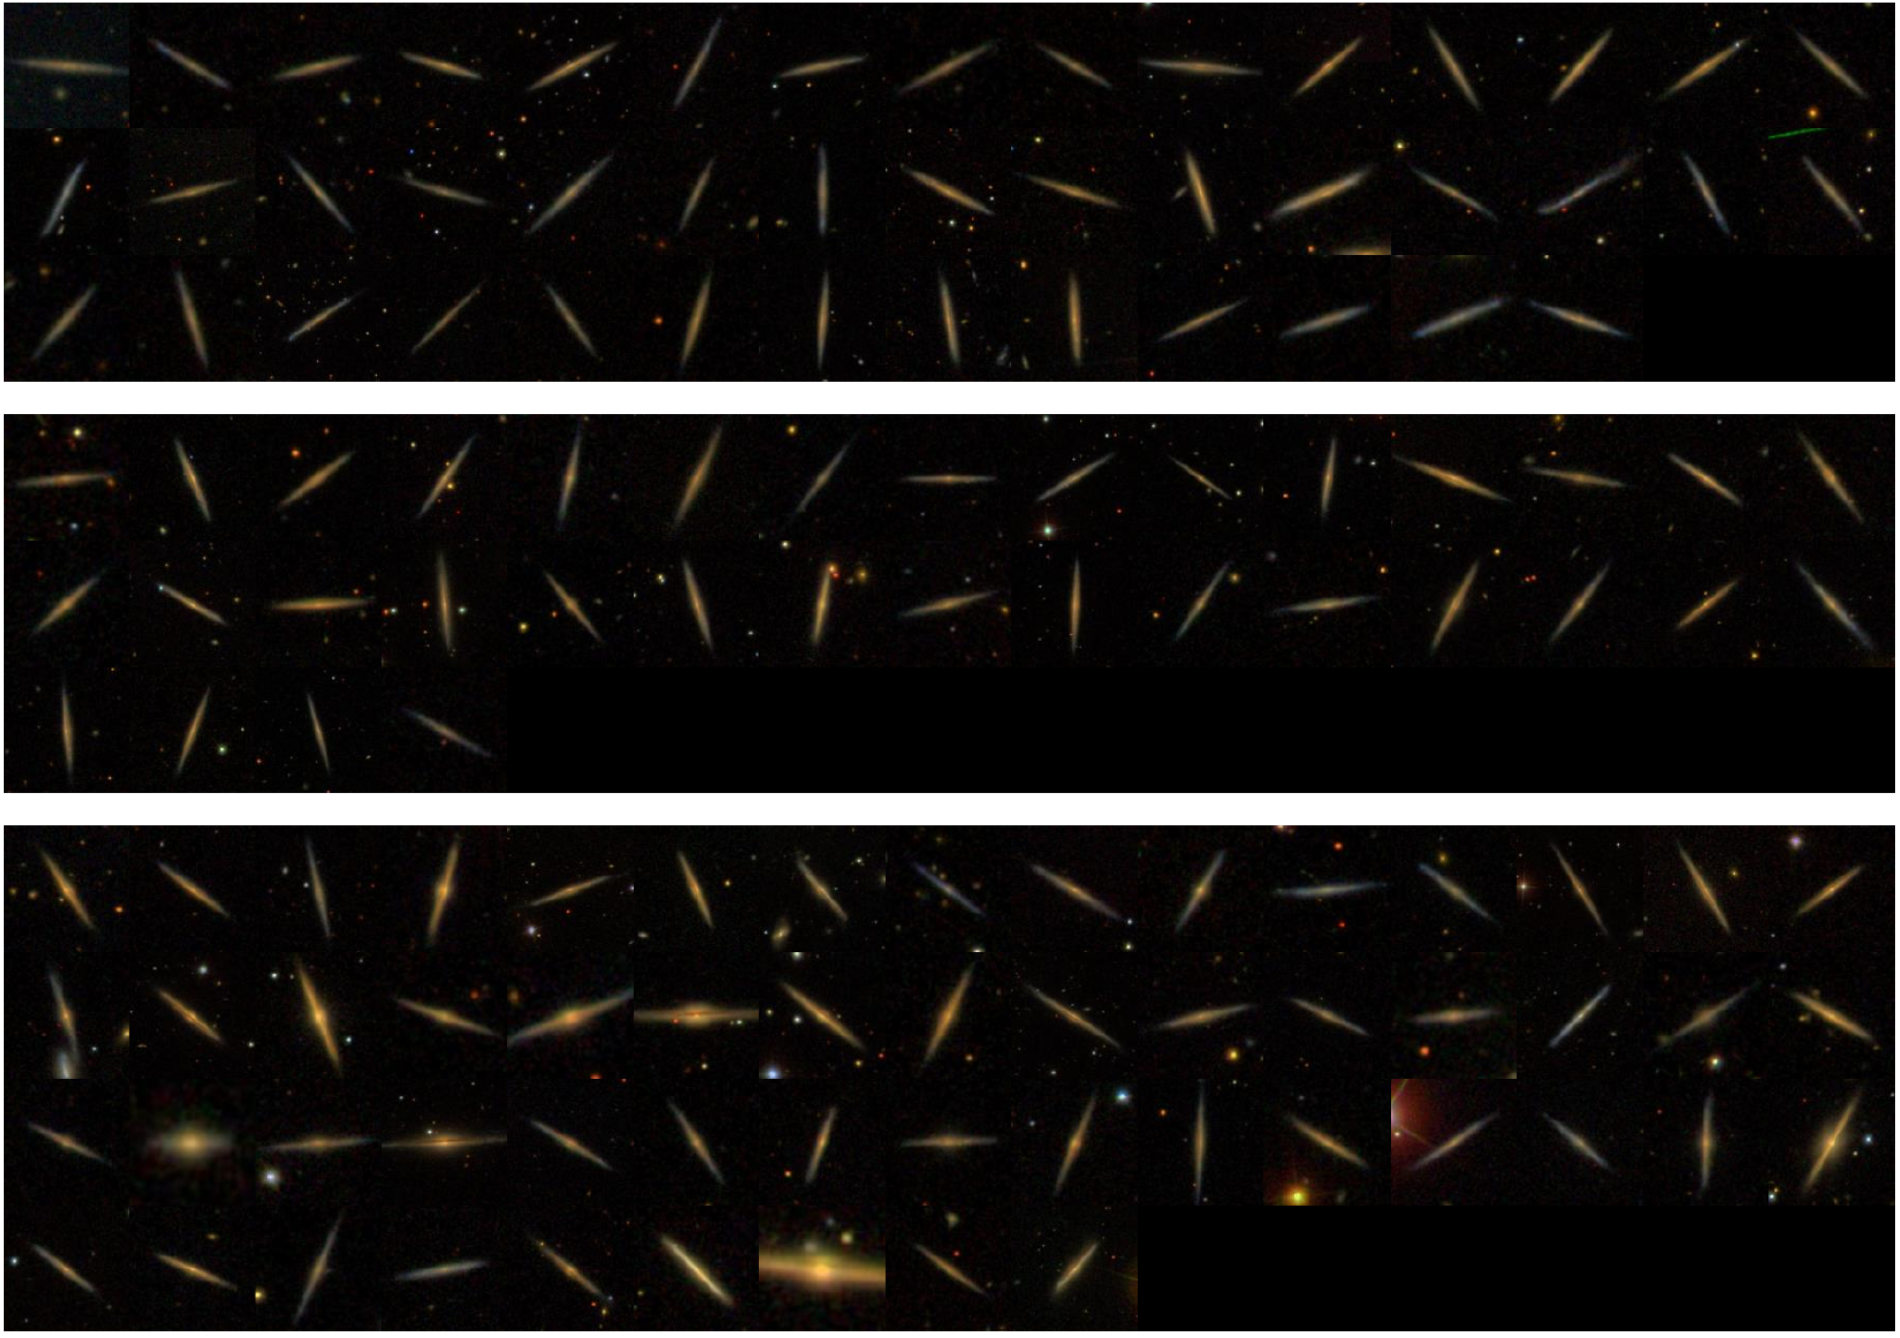
\includegraphics[width=1.0\linewidth]{pure_disk.png}
	\caption{只有盘的星系}
    \label{fig:pure-disk}
\end{figure}

盘星系的形成主要有以下步骤:
\begin{itemize}
    \item 气体落入暗物质晕,受到激波加热,形成暗物质晕中的一团热气体。
    \item 气体通过辐射冷却,降温后压强降低,气体团收缩。收缩中变热,经过几轮收缩和冷却后形成一团较密的气体团。
    \item 气体团不均匀收缩,各部分之间有相对运动,角动量逐渐转移集中,气体团开始整体性旋转。
    \item 角动量守恒让气体逐渐分布到盘上,面密度增加,密度足够高后形成恒星。
\end{itemize}

盘星系有以下统计特征:
\begin{itemize}
    \item 大的盘星系通常更亮。 如 \reffig{fig:Re-Mag} 所示。
    \item 越亮的盘星系通常更偏红。 如 \reffig{fig:red-Mag} 所示。
    \item 越亮的盘星系通常气体的占比更少。 如 \reffig{fig:gas-Mag} 所示。
    \item 越亮的盘星系转得越快, Tully-Fisher relation. (这个关系相对较明显。) 如 \reffig{fig:Tully-Fisher} 所示。
\end{itemize}

\begin{figure}[!hbtp]
	\centering 
    \subfigure[有效半径与绝对星等的关系]{
        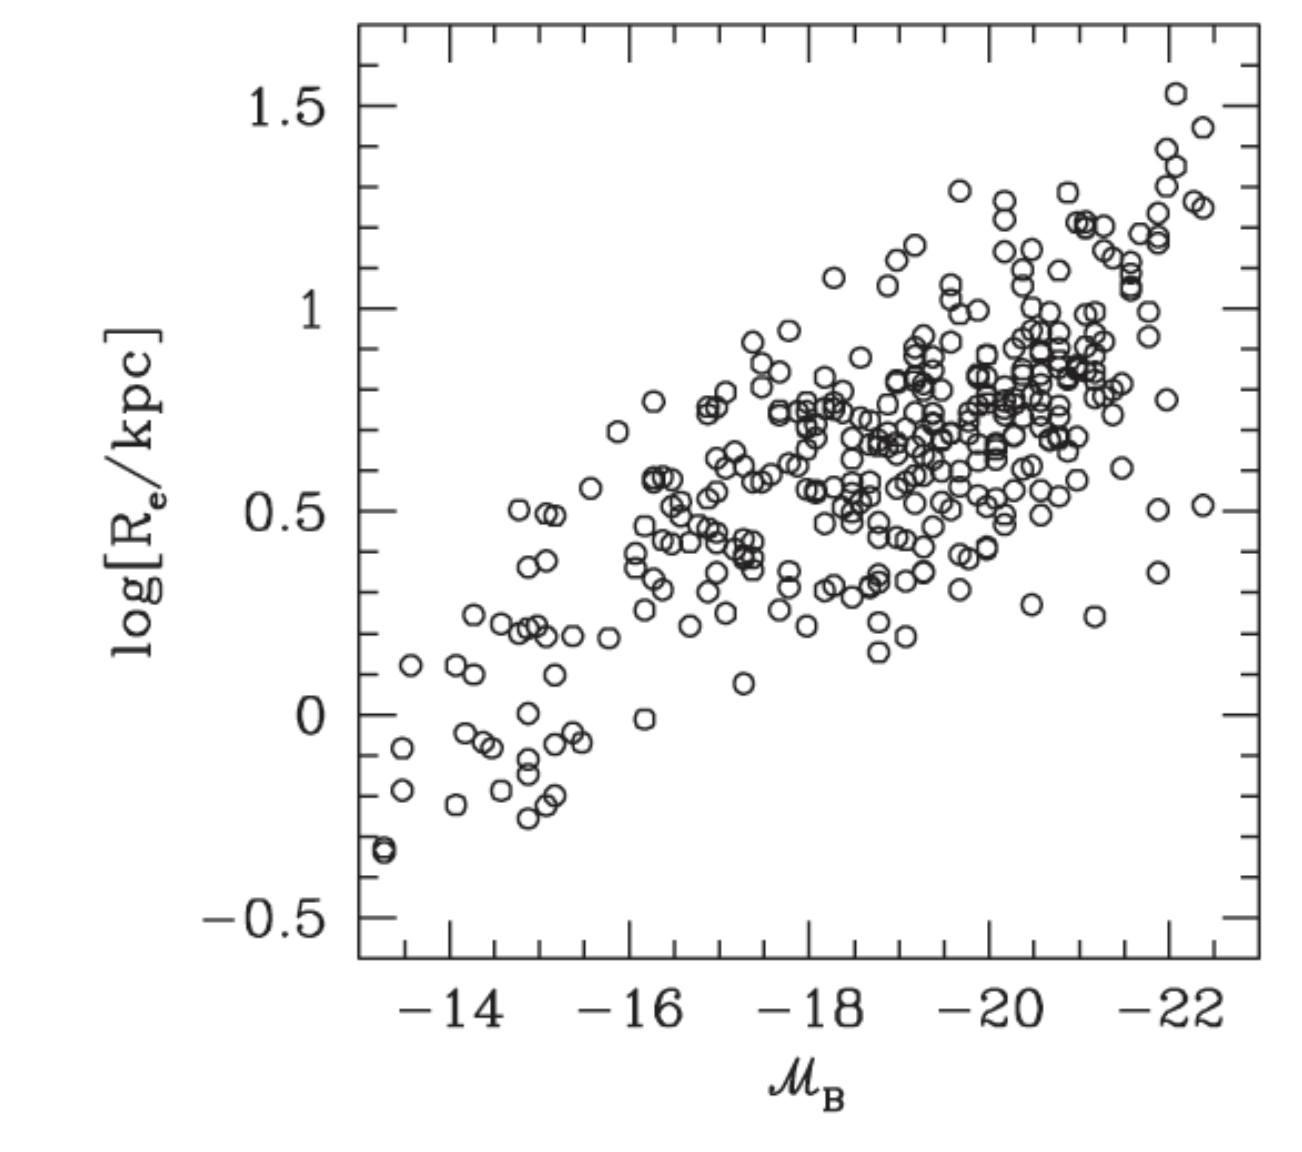
\includegraphics[width=0.4\linewidth]{Re-Mag.png}
        \label{fig:Re-Mag}
    }
    \quad
    \subfigure[色指数与绝对星等的关系]{
        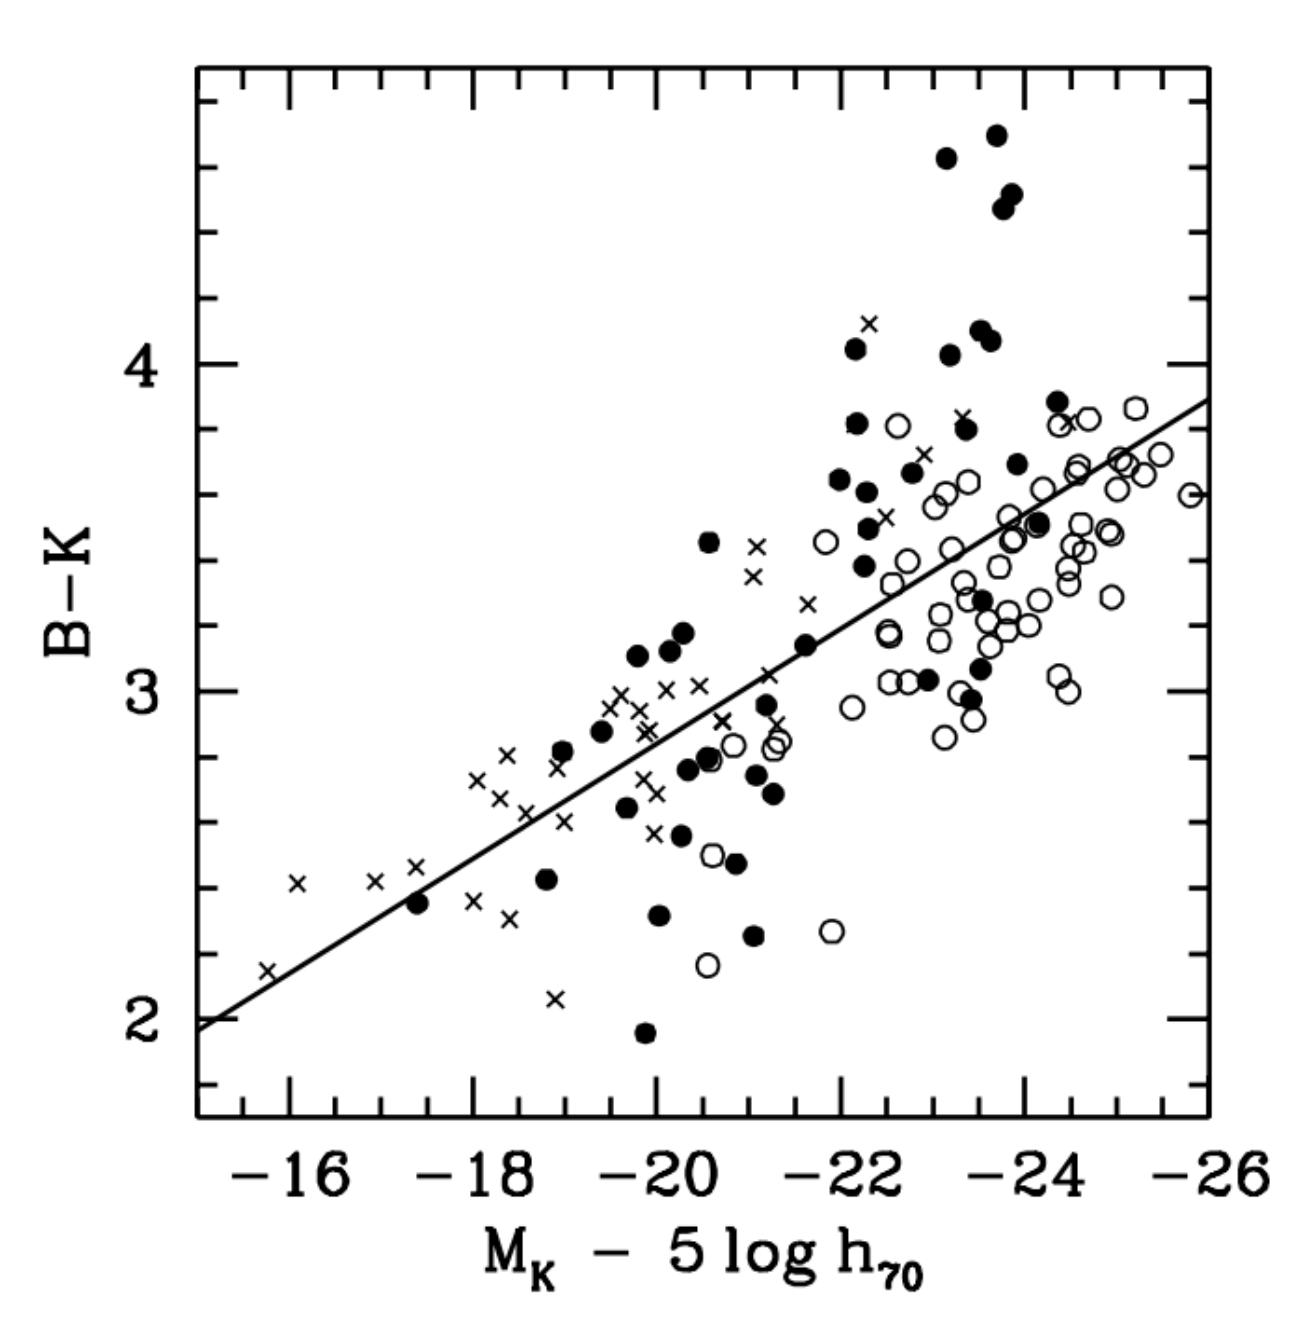
\includegraphics[width=0.4\linewidth]{red-Mag.png}
        \label{fig:red-Mag}
    }
	    
    \subfigure[气体占比与绝对星等的关系]{
        \includegraphics[width=0.4\linewidth]{gas-Mag.png}
        \label{fig:gas-Mag}
    }
    \quad	
    \subfigure[有效半径与绝对星等的关系]{
        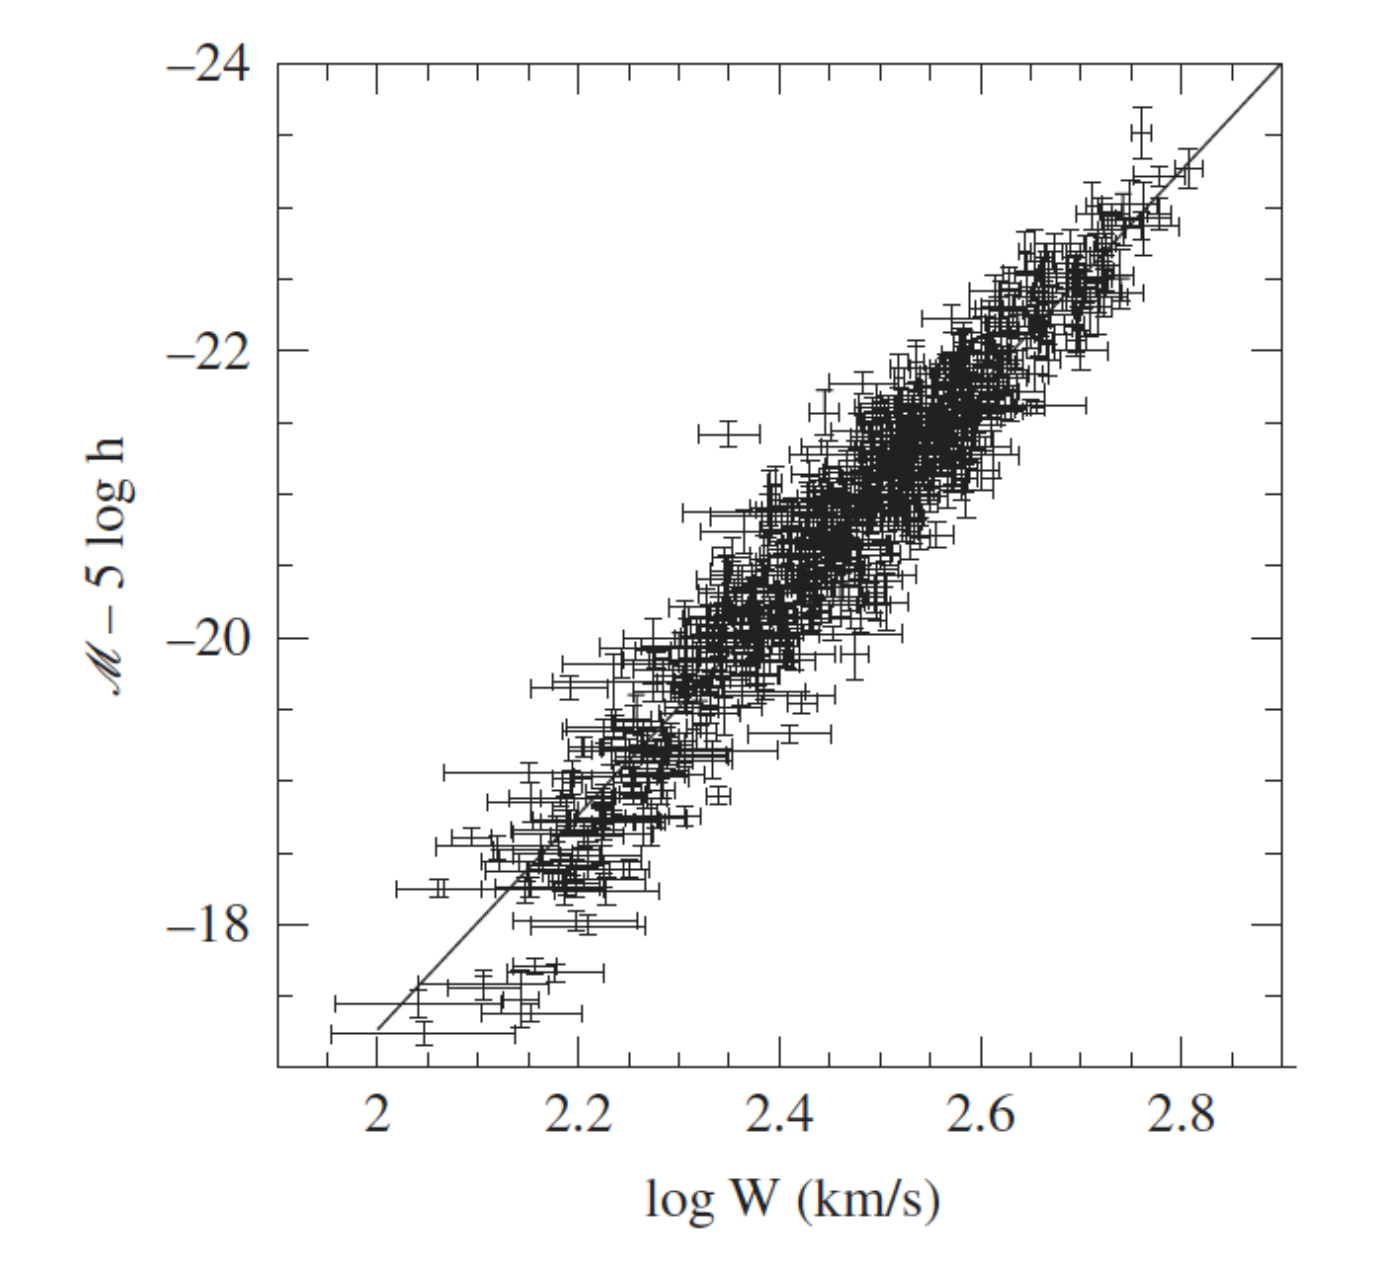
\includegraphics[width=0.4\linewidth]{TFrelation.png}
        \label{fig:Tully-Fisher}
    }
	
    \caption{盘星系的一些统计关系}
\end{figure}

\subsection{激波加热 (Shock heating)}

暗物质晕是维里化的。
气体在落入暗物质晕的过程中会与暗物质粒子相互作用,最终达到 $T _{\rm{sh}} $  温度。

假设初始气体的温度是可以忽略的,即 $v _{\rm{in}} ^2 \gg \frac{k_B T _{\rm{in}} }{\mu m_p}$.

初始能量是气体的动能 $E _{\rm{initial}} = \frac{1}{2} M _{\rm{gas}} v _{\rm{in}} ^2$

激波加热 $E _{\rm{sh}} = \frac{3}{2} N k_B T _{\rm{sh}} $
其中  $N=\frac{M _{\rm{gas}} }{\mu m_p}$ 是气体粒子的个数。

由 $E _{\rm{initial}} = E _{\rm{sh}} $,
得到 
$T _{\rm{sh}} =\frac{\mu m_p}{3k_B} v _{\rm{in}} ^2$.

对于暗物质晕来说 气体 $v _{\rm{in}} ^2 = \zeta v _{\rm{vir}} ^2$, $\zeta = \mathcal{O} (1)$ ,取决于 halo mass profile.

$T _{\rm{sh}} =\frac{\zeta \mu m_p}{3k_B} v _{\rm{vir}} ^2$


对于 被截断的奇异等温球 模型 (truncated, singular isothermal sphere of gas ),
$\zeta = 3/2$.

\begin{equation}
    T _{\rm{vir}} \equiv T _{\rm{sh}} = \frac{\mu m_p}{2k_B} v_{\rm{vir}} ^2 = 3.6\times 10^5 \mathrm{K} \left(\frac{ v_{\rm{vir}} }{100 \mathrm{~km/s}} \right) ^2
\end{equation}
定义为 维里温度。

维里温度是气体落入暗物质晕后被激波加热后所达到的温度,也用来标志一个暗物质晕可能孕育的星系在恒星形成前的气体温度。
所以,维里温度不是暗物质晕的温度,但是可以用来标志暗物质晕的性质。

\subsection{辐射冷却}

气体从高能级向低能级跃迁,辐射出光子带走能量,气体温度下降。具体的辐射机制较为复杂,本课暂不涉及。

\end{document}
